\documentclass{report}

\usepackage[utf8]{inputenc}
\usepackage[a4paper,includeheadfoot,margin=2.54cm, top=0.5in, bottom=0.5in]{geometry}
\usepackage{xcolor, hyperref, lipsum, graphicx}
\usepackage{amsmath, amsthm, amsfonts, textgreek}
\usepackage{listings}
\usepackage{color}
\usepackage{textcomp}
\usepackage{xinttools}
\usepackage{color}
\usepackage{listings}
\usepackage{caption, float}
\usepackage[most]{tcolorbox}
\usepackage{physics}

\captionsetup[lstlisting]{skip=7pt}
\renewcommand\lstlistingname{Code}
\renewcommand\lstlistlistingname{Code}

\definecolor{darkred}{rgb}{0.6,0.0,0.0}
\definecolor{darkgreen}{rgb}{0,0.50,0}
\definecolor{lightblue}{rgb}{0.0,0.42,0.91}
\definecolor{orange}{rgb}{0.99,0.48,0.13}
\definecolor{grass}{rgb}{0.18,0.80,0.18}
\definecolor{pink}{rgb}{0.97,0.15,0.45}

\definecolor{mygreen}{rgb}{0,0.6,0}
\definecolor{mygray}{rgb}{0.5,0.5,0.5}
\definecolor{mymauve}{rgb}{0.58,0,0.82}


\lstset{language=java,
aboveskip=1em,
breaklines=true,
abovecaptionskip=-6pt,
frame=single,
numbers=left,
numbersep=15pt,
numberstyle=\tiny,
backgroundcolor=\color{white},   % choose the background color
basicstyle=\footnotesize,        % size of fonts used for the code
breaklines=true,                 % automatic line breaking only at whitespace
captionpos=b,                    % sets the caption-position to bottom
commentstyle=\color{mygreen},    % comment style
escapeinside={\%*}{*)},          % if you want to add LaTeX within your code
keywordstyle=\color{blue},       % keyword style
stringstyle=\color{mymauve},     % string literal style
}


\usepackage{fancyvrb}
\usepackage{fancyhdr, lastpage}
\pagestyle{fancyplain}% <- pagestyle fancyplain
\renewcommand\plainheadrulewidth{.4pt}% headrule on plain pages
\lhead{SAE 1.02}
\rhead{S1 - Renaud \& Franceus-Cointrel}
\cfoot{Page \thepage\ of \pageref{LastPage}}
\usepackage{setspace}
\onehalfspacing


\usepackage{titlesec}


\titlespacing*{\section}
{0pt}{5.5ex plus 1ex minus .2ex}{4.3ex plus .2ex}
\titlespacing*{\subsection}
{0pt}{5.5ex plus 1ex minus .2ex}{4.3ex plus .2ex}

\title{\textbf{SAE 1.02 - E3CETE}}
\author{J. Renaud - M. Franceus-Cointrel}
\date{Pour le 14 janvier 2024}


\addtolength{\jot}{1em}

\hypersetup{
  pdftitle={SAE 1.02 : E3Cete - 2023/2024},
  pdfauthor={Renaud Julien, Franceus-Cointrel Milwenn},
  pdfsubject={Dev. Init.}
}

\renewcommand{\contentsname}{Table des matières}
\renewcommand{\appendixname}{Annexe}
\renewcommand{\chaptername}{Chapitre}


\begin{document}

\maketitle
\tableofcontents

\chapter*{Introduction}

\qquad Dans cette SAE nous étudions...




\chapter{Analyse et comparaison des 3 méthodes de tris}

\qquad 

\section{Les fonctions de tris et comptage du nombre d'opérations approximatif}

\subsection{Tri par sélection}

\begin{lstlisting}[language=java, caption={\it Focntion marche aléatoire}, label=code1]
%insert code here
\end{lstlisting}

\subsection{Tri par bulles}

\subsection{Tri par insertion}

\pagebreak



\section{Protocole de test}

\subsection{Définition des variables}

L'objectif de cette expérience est d'évaluer la performance de chacun des tris. Pour cela nous devons réaliser chacun des tris en variant le nombre de cartes $N$ contenus dans le Paquet. Pour cette expérience les paquets triés seront toujours pleins, et le nombre de cartes $N$ contenus est déterminé par les cardinalités des caractéristiques possibles. En principe nous fixons les cardinalités associés aux couleurs/figures/textures pour ne seulement varier le nombres de répétition des figures. Ainsi $N$ est défini tel que : 

\begin{equation*}
	N = cardCouleurs \times cardFigures \times cardTextures \times cardRepetFigures
\end{equation*}

\bigskip

\noindent Pour chacun des méthodes de tris nous calculons le nombre d'opération $nOpApprox$ et son temps d'éxecution (en ms) $tempsExec$. Ainsi, en répétant les tris $nbRepetTest$ nombre de fois pour $N$ fixé, nous en déduisions les valeurs moyennes ainsi que leurs incertitudes (écartype) telles que :

\boldmath
\begin{equation} \label{eq:1}
nbOpMoy = \dfrac{1}{nbRepetTest} \times \sum_{i = 1}^{nbRepetTest} nbOpApprox_{i}
\end{equation} 
\begin{equation} \label{eq:2}
	u\_nbOp = \sqrt{\dfrac{1}{nbRepetTest} \times \sum_{i = 1}^{nbRepetTest} (\,nbOpApprox_{i} - nbOpMoy)\,^{2}}
\end{equation} 
\begin{equation} \label{eq:3}
	tempsExecMoy = \dfrac{1}{nbRepetTest} \times \sum_{i = 1}^{nbRepetTest} tempsExec_{i}
\end{equation} 
\begin{equation} \label{eq:4}
	u\_tempsExec = \sqrt{\dfrac{1}{nbRepetTest} \times \sum_{i = 1}^{nbRepetTest} (\,tempsExec_{i} - tempsExecMoy)\,^{2}}
\end{equation} 
\unboldmath

\subsection{Protocole expérimental}

\begin{enumerate}
	\item Réaliser les 3 tris sur $nbRepetTest$ paquets ayant les mêmes caractéristiques mais chacun mélangés différemment, pour un même nombre de cartes $N$.
	\item Récupérer le nombre d'opération $nbOpApprox$ et le temps d'éxécution $tempsExec$ de chacun des tris pour toutes les répétitions.
	\item Calculer et stocker les valeurs moyennes $nbOpMoy$ (\ref{eq:1}) et $tempsExecMoy$ (\ref{eq:3}), ainsi que leurs incertitudes $u\_nbOp$ (\ref{eq:2}) et $u\_tempsExec$ (\ref{eq:4}).
	\item Répéter l'expérience en variant $N$, en modifiant la valeur de $cardRepetFigures$.
\end{enumerate}


\subsection{Fonctions Test}

\begin{lstlisting}[language=java, caption={\it Focntion marche aléatoire}, label=code2]
%insert code here
\end{lstlisting}



\newpage
\section{Test n°1}
\subsection{Initialisation et spécificités}
Les variables :
\begin{itemize}
	\item int $nbRepetTest = 1000$
	\item int $cardCouleurs = 1$
	\item int $cardFigures = 1$
	\item int $cardTextures = 1$
	\item int $cardRepetFigures \in [\, 10-500 ]\, $
\end{itemize}
Specificités de l'appareil utilisés : ...........



\subsection{Analyse graphique}

\qquad Nous stockons les données des tests sous forme de 3 fichiers .csv, grâce à une fonction de conversion. Chaque fichier correspond à une méthode de tri et contient toutes les valeurs de $N$, $nbOpMoy$, $u\_nbOp$, $tempsExec$, $u\_tempsExec$ associées à cette dernière. Nous choisissons de réaliser le graphique de $nbOpMoy=f(\,N)\,$ et de $tempsExecMoy=f(\,N)\,$ à l'aide du logiciel \href{https://regressi.fr/WordPress/}{\it \underline{Regressi}}.

\bigskip

\noindent Etant donées que ces 3 fonctions de tris utilisent chacune une double boucle imbriquée, nous nous attendons à une complexité quadratique $O(\,n^2\,)$.

\begin{figure}[H]
	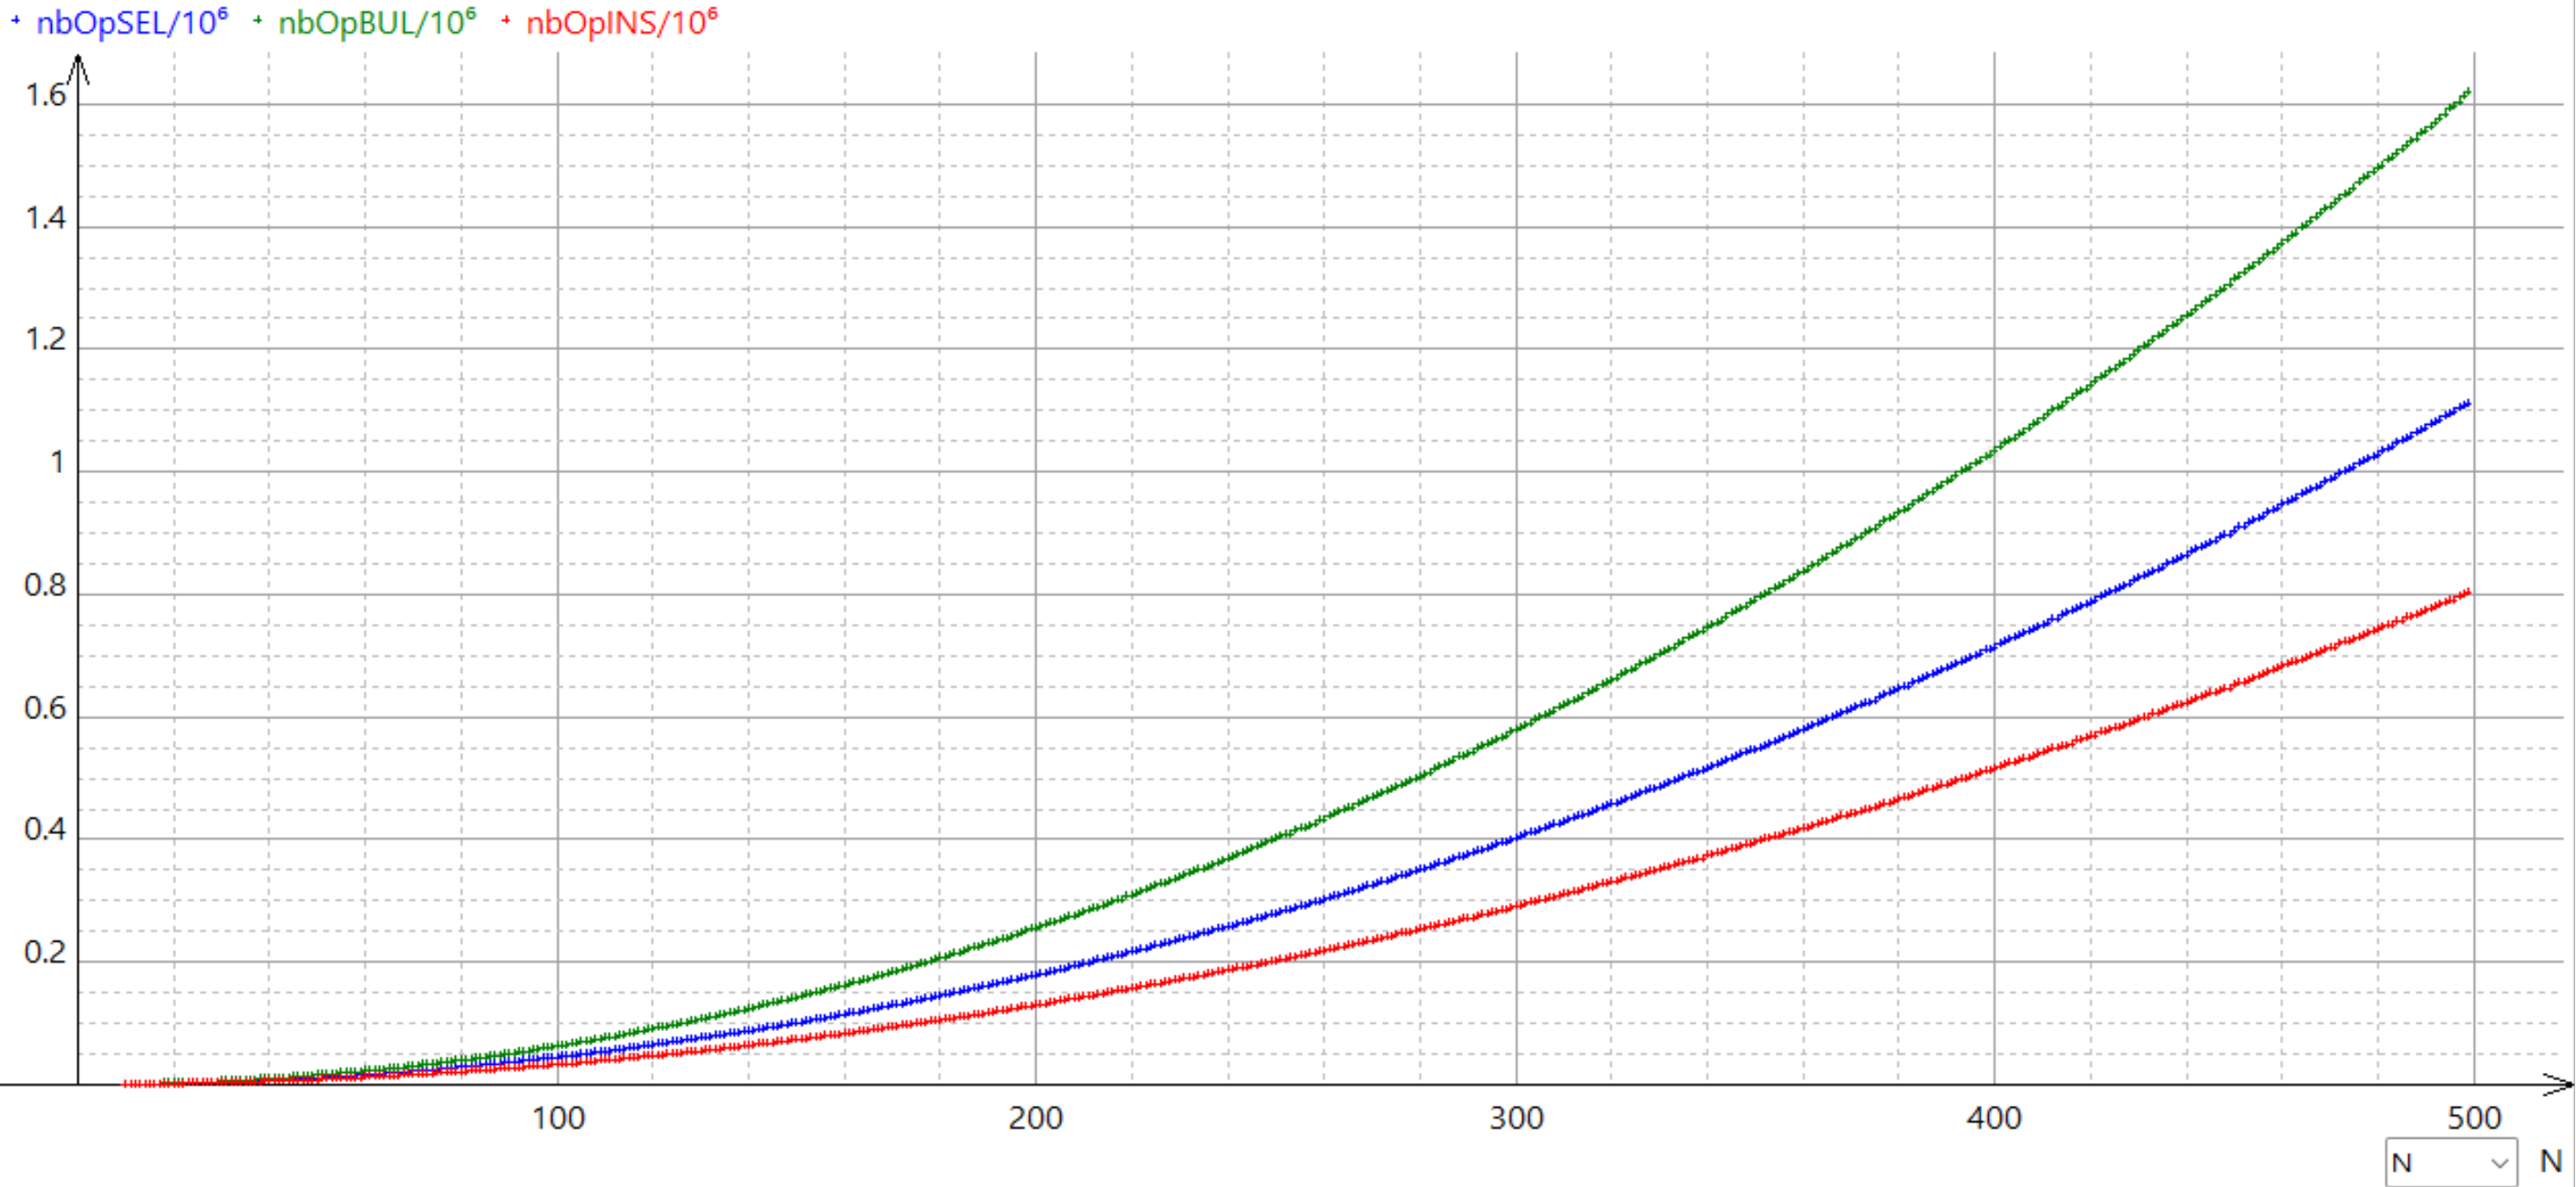
\includegraphics[width=\textwidth]{../graphe/graph1.png}
	\caption{Graphique de $nbOpMoy=f(\,N)\,$ pour les 3 méthodes de tris : en bleu .............}
\end{figure}
\begin{figure}[H]
	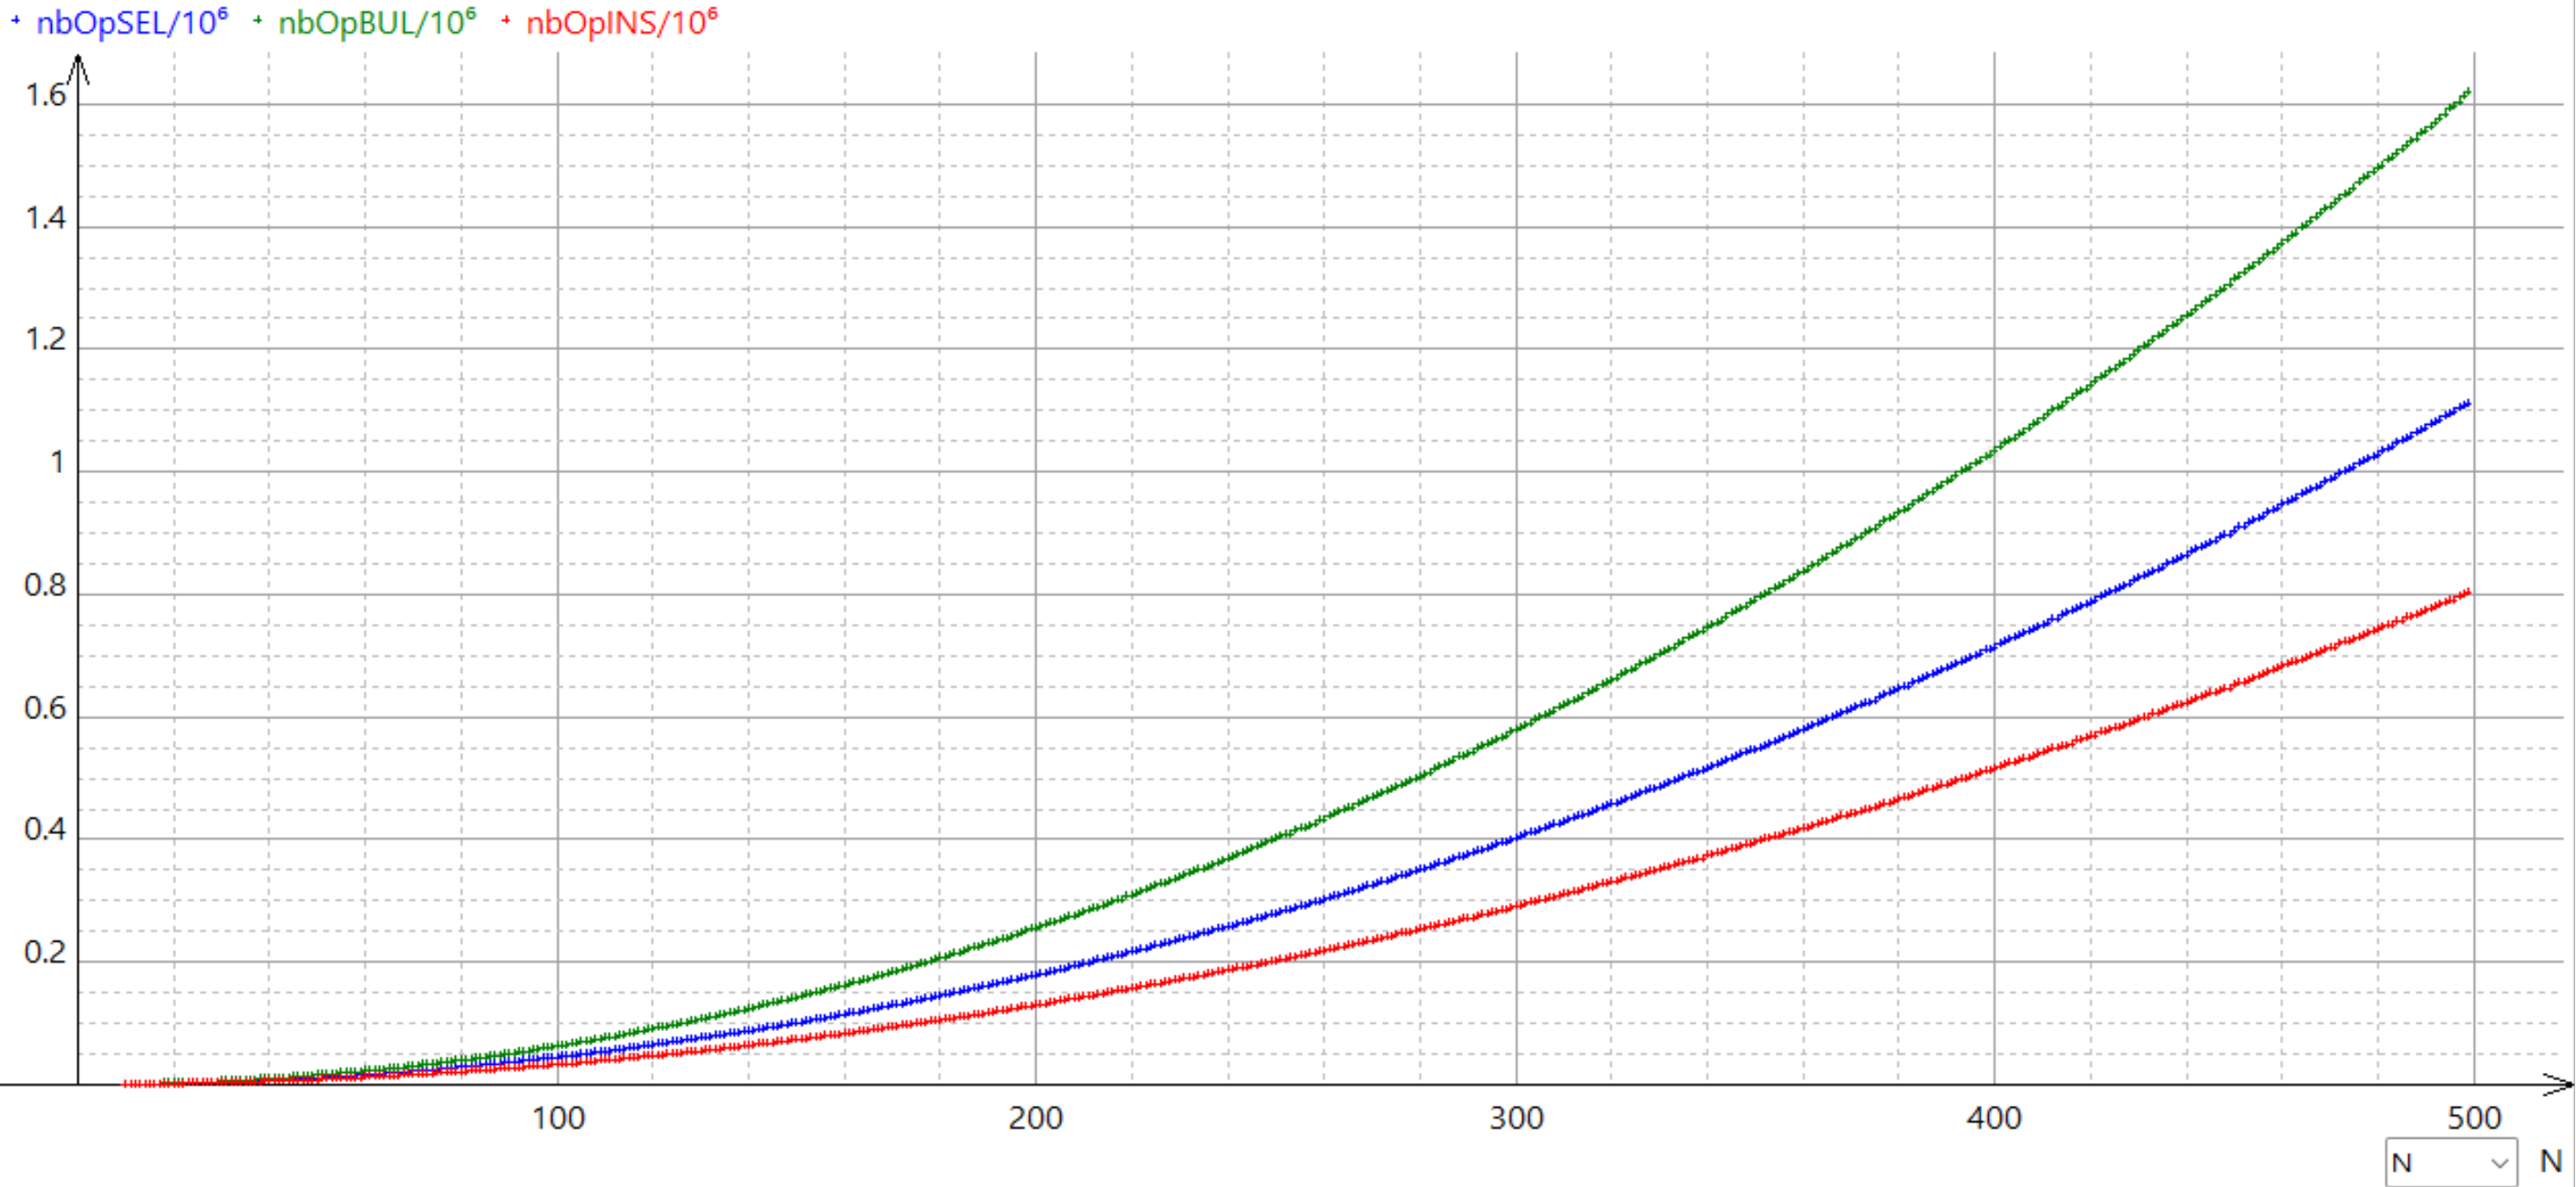
\includegraphics[width=\textwidth]{../graphe/graph1.png}
	\caption{Graphique de $tempsExecMoy=f(\,N)\,$ pour les 3 méthodes de tris : en bleu .............}
\end{figure}

Commentaire : ........................................................................




\chapter{Théorie}

\section{Représentation mathématique de la Class \it Table}

\begin{enumerate}
	\item Une \textit{Table} est une liste ordonée de \textit{Cartes} tous différentes (pas de répétition), parmi toutes les \textit{Cartes} du jeu contenues dans un \textit{Paquet}. Une \textit{Table} est donc un arrangement. 
	
	\item Pour une \textit{Table} de 9 \textit{Cartes} et un jeu de 81 \textit{Cartes}, le nombre de \textit{Tables} différentes possibles est tel que : 
	\bigskip
	$$A^{9}_{81} = \frac{81!}{(81-9)!} = 81\times80\times...\times74\times73 = 94670977328928000$$
	
\section{Etude du cas 3CR}
\subsection{Calculs théoriques}
	\item Sachant que pour une \textit{Carte} il y a 3 \textit{Couleurs}, 3 répétitions maximales de figures, 3 \textit{Figures} et 3 \textit{Textures} possibles ; on en déduit qu'il existe $1\times3\times3\times3=27$ cartes rouges distinctes. Pour déterminer les arrangements possibles contenant exactement 2 cartes rouges, nous comptons le nombre de combinaisons possibles de 3 cartes rouges parmi les 27 que multiplie le nombre de combinaisons possibles des 6 cartes restantes de la \textit{Table} parmi les 54 cartes non rouges. A chacune de ces combinaisons possibles de 3 cartes rouges + 6 cartes non rouges (pas d'ordre), nous pouvons réaliser $9!$ permutations possibles. Ainsi, le nombre de \textit{Tables} différentes contenant exactement 3 \textit{Cartes} rouges est tel que :	
	$$C^{3}_{27} \times C^{6}_{81-27} \times 9! = \frac{27!}{3!(27-3)!} \times  \frac{54!}{6!(54-6)!} \times 9! = 2925 \times 25827165 \times 362880 = 27413572782960000$$

	\item On en déduit la probabilité $P_{3CR}$ d'obtenir une \textit{Table} contenant exactement 3 cartes rouges :
	$$P_{3CR} = \dfrac{casFavorables}{casTotal} = \dfrac{C^{3}_{27} \times C^{6}_{81-27} \times 9!}{A^{9}_{81}} = \dfrac{27413572782960000}{94670977328928000} = 0.28956680871386137 $$

\subsection{Fonction \textit{proba3RC}}
	\item fonction here


\subsection{Traitements de données et analyse graphique}
\begin{figure}[H]
	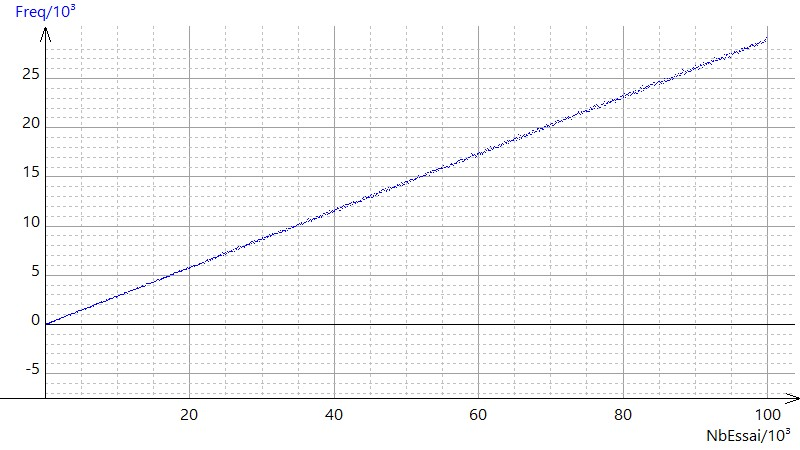
\includegraphics[width=\textwidth]{../graphe/Freq(n).jpg}
	\caption{Graphique de $Freq=f(nbEssai)$ en faisant varier $nbEssai$ de 100 à 100 000 par pas de 100}
\end{figure}	
\bigskip

Les graphiques obtenus à partir des données générées par cette fonction permettent de déterminer une valeur expérimental de $P_{3CR}exp$. En effet, en traçant $Freq=f(nbEssai)$ nous apercevons que la courbe varie linéairement. Ceci est en accord avec la théorie puisque $P_{3CR}theo = \dfrac{casFavorables}{casTotal}$ soit $casFavorables = P_{3CR}\times casTotal$ ce qui équivaut à  $Freq=a\times nbEssai$. En réalisant une modélisation linéaire grâce à l'outils de modélisation sur le logiciel \href{https://regressi.fr/WordPress/}{\it \underline{Regressi}} ; nous en déduisons : 
$$P_{3CR}exp = a = 0.28939 \pm 0.00015$$
Nous pouvons calculer le pourcentage d'erreur $Err$ telle que :
$$Err = abs\left(\dfrac{P_{3CR}theo - P_{3CR}exp}{P_{3CR}theo}\right) \times100 = 0.061\%$$	

	\item fonction here
	
Pour déterminer à partir de combien d'essais il faut pour obtenir un résultat fiable, nous avons choisi de tracer $Err=f(nbEssai)$ à partir des probabilités propres à chacun des événements (associé à nombre d'essais) : $P = Freq/nbEssai$.
\begin{figure}[H]
	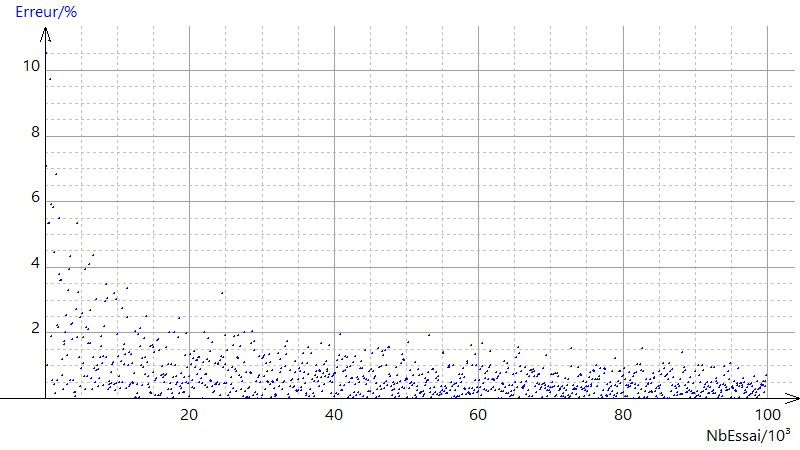
\includegraphics[width=\textwidth]{../graphe/Erreur(n).jpg}
	\caption{Graphique de $Err=f(nbEssai)$ en faisant varier $nbEssai$ de 100 à 100 000 par pas de 100}
\end{figure}	
Nous observons que pour avoir un résultat fiable à 5\% d'erreur près, il faut au moins environ 10 000 essais. Le graphique ci-dessous de $P=f(nbEssai)$ illustre bien la répartition des probabibilités qui converge vers la valeur théorique en augmentant le nombre d'essais. 
\begin{figure}[H]
	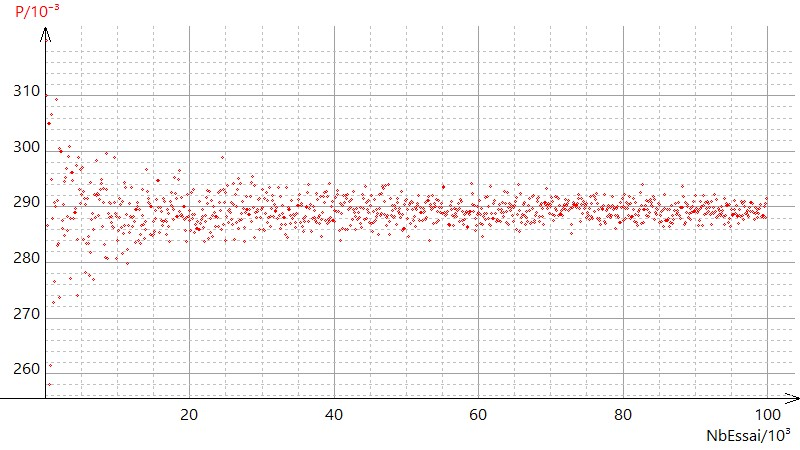
\includegraphics[width=\textwidth]{../graphe/P(n).jpg}
	\caption{Graphique de $P=f(nbEssai)$ en faisant varier $nbEssai$ de 100 à 100 000 par pas de 100}
\end{figure}	

\section{Etude du cas 3CR\&2CL}

\subsection{Caluls théoriques}
	\item L'intersection de l'ensemble des cartes rouges et des cartes ayant au moins un losange n'est pas vide. Il faut étudier chacune des cas. Il y a 27 cartes rouges distincts et 27 cartes ayant au moins un losange. Parmi ces cartes rouges seulement $1\times3\times2\times3=18$ n'ont pas de losange. De même, parmi les cartes ayant au moins un losange, $2\times3\times1\times3=18$ ne sont pas rouges. Ainsi, $1\times3\times1\times3=9$ cartes sont à la fois rouges et ont au moins un losange. 
\bigskip
\begin{table}[H]

\caption{Tableau récapitulatif des différents cas possibles pour obtenir une combinaison de 9 cartes avec exactement 3 cartes rouges et 2 cartes ayant au moins un losange :}
\end{table}



\bigskip
On en déduit le nombre d'arrangements possibles de \textit{Table} contenant exactement 3 cartes rouges et 2 cartes ayant au moins 1 losange tel que :

\begin{align*}
9! &\times(\,C^{2}_{9} \times C^{1}_{18} \times C^{0}_{18} \times C^{6}_{36} \\
&+C^{1}_{9} \times C^{2}_{18} \times C^{1}_{18} \times C^{5}_{36} \\
&+C^{0}_{9} \times C^{3}_{18} \times C^{2}_{18} \times C^{4}_{36} )\, \\
&= 362880 \times 17960464368 = 6517493309859840
\end{align*}

On en déduit la probabilité $P_{3CR\&2CL}$ de cet événement :
	$$P_{3CR\&2CL} = \dfrac{casFavorables}{casTotal} = \dfrac{6517493309859840}{94670977328928000} = 0.06884362550959248 $$


\subsection{Vérification empirique succincte}
\item fonction here

\section{Etude du cas E3C}

\subsection{Methode \textit{estUnE3C}}
\subsection{Traitements de données et analyse graphique}


\end{enumerate}
























\appendix
\chapter{Modules utilisés}

\begin{lstlisting}[caption={\it Modules utilisés en Python 3.9.2}, label=annexe]
  import math
    from math import pi
  import random as rnd
  import statistics as stats
  import matplotlib
  import matplotlib.pyplot as plt
  import matplotlib.cm as cm
    from matplotlib.patches import Ellipse
    from mpl_toolkits import mplot3d
  import numpy as np
  import scipy as scp
  import scipy.stats as st
    from scipy.stats import multivariate_normal

\end{lstlisting}

\chapter{Sources}

\begin{itemize}
  \item \url{https://moodle.umontpellier.fr/course/view.php?id=25363}
  \item \url{https://femto-physique.fr/physique_statistique/diffusion-moleculaire.php}
  \item \url{https://stringfixer.com/fr/Random_walk}
  \item \url{https://en.wikipedia.org/wiki/Mass_diffusivity}
  \item \url{https://fr.wikipedia.org/wiki/Mouvement_brownien}
  \item \url{https://fr.wikipedia.org/wiki/Lois_de_Fick}
  \item \url{https://fr.wikipedia.org/wiki/Cha%C3%AEne_id%C3%A9ale}
  \item \url{https://fr.wikipedia.org/wiki/Loi_multinomiale}
  \item \url{https://en.wikipedia.org/wiki/Multivariate_normal_distribution}
  \item \url{https://www.youtube.com/channel/UCmpptkXu8iIFe6kfDK5o7VQ}
  \item \url{https://www.caam.rice.edu/~heinken/latex/symbols.pdf}
  \item \url{https://matplotlib.org/stable/index.html}
\end{itemize}

\begin{figure}
  \centering

  \caption{\it Langages et éditeurs utilisés}
\end{figure}





\end{document}









